\section{Introductie}
\subsection{De opdracht}
Er is aan ons gevraagd om een omroepspeaker te ontwerpen. Onze taak is om een versterker te maken een 8Ω speaker (deze is vooraf aangeleverd). 

\subsection{Onze aanpak}
Om te beginnen stellen we als doel om aan de basiseisen van de opdracht te voldoen omdat we van ons zelf niet weten hoe goed we zijn in dit onderwerp. Wanneer blijkt dat we als groep een grotere uitdaging aankunnen zullen we dit bespreken met elkaar en de Docent-begeleider en vervolgens mogelijk excelleren. 

\begin{figure}[h]
    \centering
    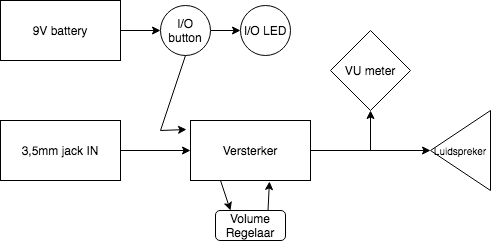
\includegraphics[width=0.75\textwidth]{diagram}
    \caption{diagram}
    \label{fig:diagram}
\end{figure}

\subsection{Wat te doen bij conflicten/niet functioneren}
Bij het niet-functioneren van een student kan de projectgroep besluiten een waarschuwing te geven. Deze waarschuwing wordt per email gestuurd naar het hhs mailadres van het groepslid met een cc naar alle andere groepsleden en de docent-begeleider.
Als er op deze manier een tweede formele waarschuwing door de projectgroep gegeven wordt kan de docent gevraagd worden bij het eerstvolgende toetsmoment een deelcijfer 0 te geven. In een derde formele waarschuwing kan de docent gevraagd worden om een NVD als eindoordeel te geven. NVD betekent Niet Voldaan. Het project is dan voor deze student afgelopen.
De projectgroep is bereid serieus naar het verhaal van de beklaagde te luisteren en kan een waarschuwing intrekken als de conclusie wordt getrokken dat de waarschuwing niet terecht was.
